\documentclass{beamer}

\usetheme{CambridgeUS}
\usecolortheme{orchid}

\usepackage{graphicx}
\usepackage{tikz}
\usepackage{listings}
\usepackage{colortbl}
\usepackage{color}


\tikzstyle{block} = [rectangle, draw, text width=4.5em, text centered, minimum height=2em]
\lstset{basicstyle=\small\ttfamily}



\lstset{
  language=Java,
  basicstyle=\ttfamily\small,
  keywordstyle=\color{blue},
  commentstyle=\color{green!60!black},
  stringstyle=\color{red},
  showstringspaces=false,
  breaklines=true
}


\definecolor{mygray}{rgb}{0.5,0.5,0.5}
\definecolor{mygreen}{rgb}{0,0.6,0}
\definecolor{myblue}{rgb}{0,0,0.8}
\lstset{language=XML,
        morekeywords={m:GetPrice, m:StockName},
        basicstyle=\ttfamily,
        keywordstyle=\color{myblue},
        commentstyle=\color{mygreen},
        stringstyle=\color{myblue},
        numbers=left,
        numberstyle=\tiny\color{mygray},
        stepnumber=1,
        numbersep=3pt,
        backgroundcolor=\color{white},
        tabsize=1,
        showspaces=false,
        showstringspaces=false
}

% Define Protobuf language
\lstdefinelanguage{protobuf}{
  keywords={message, optional, repeated, required, string, int32, bool},
  keywordstyle=\color{blue}\bfseries,
  ndkeywords={bool, int32, float, double, string},
  ndkeywordstyle=\color{darkgray}\bfseries,
  identifierstyle=\color{black},
  tabsize=1,
  sensitive=false,
  comment=[l]{//},
  morecomment=[s]{/*}{*/},
  commentstyle=\color{purple}\ttfamily,
  stringstyle=\color{red}\ttfamily,
  morestring=[b]",
  morestring=[b]',
}

\definecolor{codegray}{gray}{0.9}
\newcommand{\code}[1]{\colorbox{codegray}{\texttt{#1}}}


\setbeamertemplate{navigation symbols}{} % Remove navigation symbols

\title{API Design and Management}
\author{Mohamed Sweelam}
\institute{Software Engineer}
\date{}

% Add the title graphic here
\titlegraphic{
\includegraphics[width=7cm, height=3.5cm]{img/course-logo.png}}
\logo{
\includegraphics[height=1cm]{img/channel-logo-circular.png}}

\begin{document}

\begin{frame}
  \titlepage
\end{frame}

\begin{frame}{Outline}
  \tableofcontents
\end{frame}

\section{Course Objectives}
\begin{frame}
	\frametitle{Course Objectives} % Table of contents slide, comment this block out to remove it
		\begin{enumerate}
			\item<1-> Provide good Arabic content for the topic
			\item<2-> Overview of API Design and Management
			\item<3-> Role and Importance of APIs in Distributed Systems
			\item<4-> The best practices you should follow today
		\end{enumerate}
\end{frame}

\section{Understanding APIs}
\begin{frame}{Understanding APIs}
	\begin{block}{Definition \tiny{\textit{wikipedia}}}
		\small{ Application programming interface (API) is a way for two or more computer programs or components to communicate with each other. It is a type of software interface, offering a service to other pieces of software.}
	\end{block}
	
	\begin{block}{Definition \tiny{\textit{ChatGPT}}}
		\small{ API (Application Programming Interface) is a set of rules, protocols, and tools for building software applications. It specifies how software components should interact and is used to enable the integration between different software systems. }
	\end{block}
	
	\begin{alertblock}{History \tiny{\textit{wikipedia}}}
		\small{ The term "application program interface" is first recorded in a paper called Data structures and techniques for remote computer graphics in 1968. The authors use the term to describe the interaction of an application "Graphics Program" with the rest of the computer system. }
	\end{alertblock}
  
\end{frame}

\begin{frame}{Understanding APIs \small{\textit OSI Model}}
	\small {The open systems interconnection (OSI) model is a conceptual model created for Standardization which enables diverse communication systems to communicate using standard protocols.} 
	\begin{center}
    		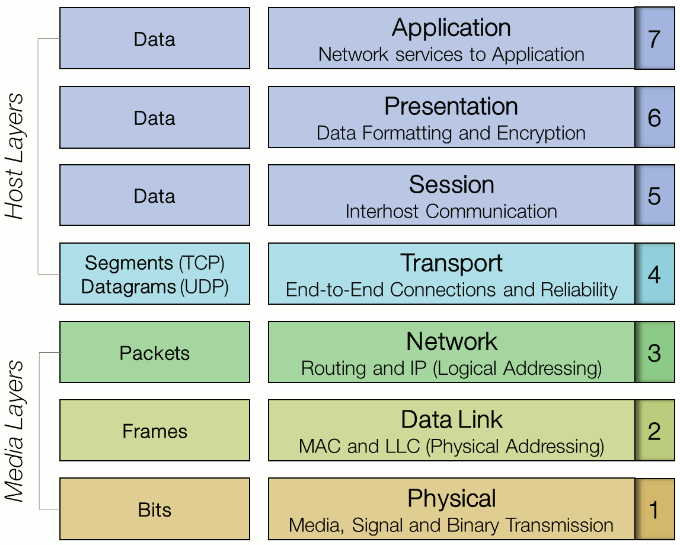
\includegraphics[width=0.8\textwidth, height=0.6\textheight]{img/osi-model.png}
  \end{center}
  \tiny { source: \href{https://www.coengoedegebure.com/osi-model}{\textcolor{blue}{coengoedegebure.com/osi-model}}}
\end{frame}

\begin{frame}{Understanding APIs \small Example}
	\begin{center}
    		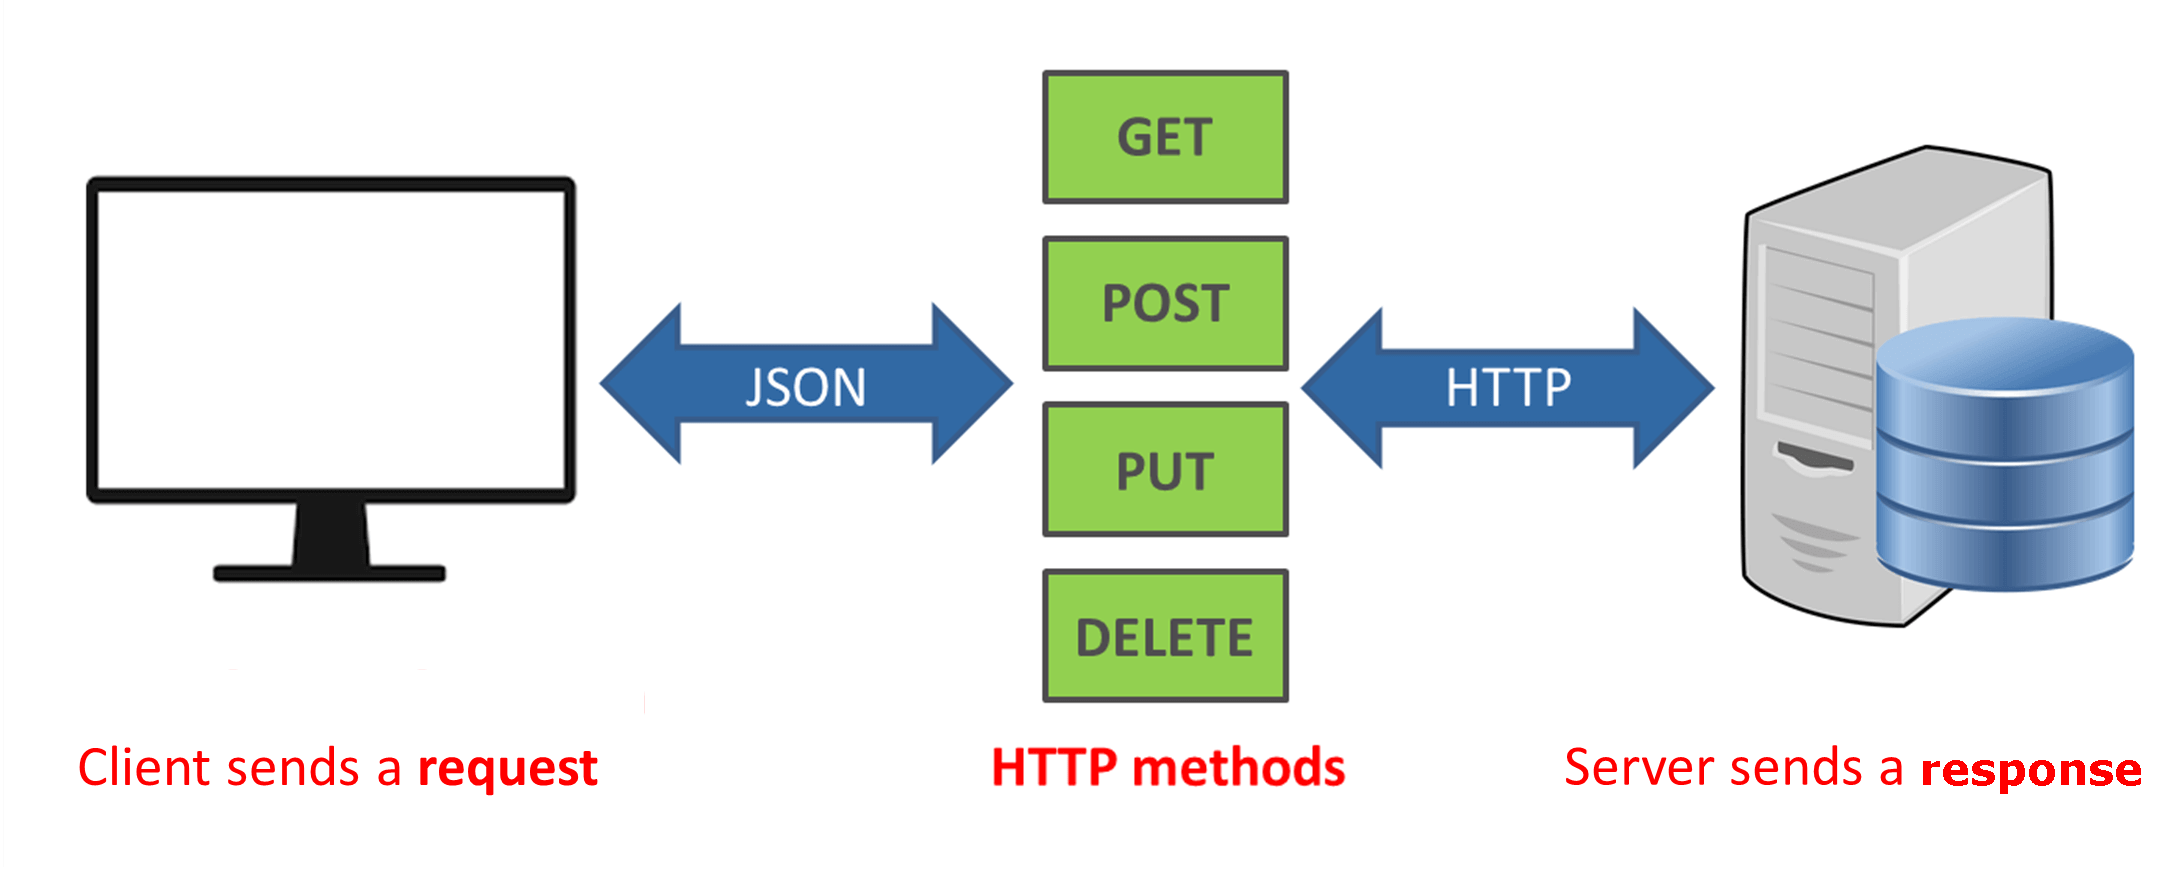
\includegraphics[width=0.6\textwidth, height=0.4\textheight]{img/api-client-to-server.png}
  \end{center}
  
  \tiny { source: \href{https://phpenthusiast.com/blog/what-is-rest-api}{\textcolor{blue}{phpenthusiast.com/blog/what-is-rest-api}}}
\end{frame}

\begin{frame}[t]{Understanding APIs \small (API Types)}
  There are several types of API, each one serves specific use case.
  
  \begin{itemize}
  	\item<1-> Public APIs (Open APIs) \\
  	\tiny{ The APIs are publicly available and can be designed in various ways, taking security into account. However, \underline{the main priority is to ensure they are easily consumable by as many clients as possible. }}

  	\item<2-> \small Partner APIs \\
  	\tiny{ Specialized interfaces that enable organizations to access data and service offerings across businesses (B2B) in order to create unique features within their own applications or services by utilizing a partner's resources. }
  	
  	\item<3-> \small Internal APIs \\
  	 \tiny{ Intended for use internally by the organizations own developers. These APIs facilitate the transmission of data between different components of a system, enabling process automation. }
  	 
  	\item<4-> \small Composite APIs  {\tiny Executes a series of API requests in a single call.}
  	\vspace{3mm}
    \item<5->[] The types can be designed and developed using two ways \\
    \begin{enumerate}
     \item API Architectural Style, 
     \item API Standard Protocol.  
    \end{enumerate}    
  \end{itemize}   
  
  
\end{frame}


\begin{frame}[t]{Understanding APIs \small (API Architecture vs API Protocols)}
  \begin{block}{API Architecture Style}  
   \scriptsize It refers to the high-level structural design of the API. It encompasses the standards, and best practices governing how the API is developed, how it interacts with other systems, and how it exposes its functionality and data.\\
   \color{teal} Example: REST
  \end{block}
  
  \begin{alertblock}{No Restrictions}
    \scriptsize Architectural style is sensitive to change and enhancement; it relies more on human experience.
  \end{alertblock}
  
  
  \begin{block}{API Protocol}
    \scriptsize It refers to a set of rules and standards used for communication between various software components. The protocol dictates how requests and responses are formatted and transmitted, and what are the restrictions of the communication.\\
    \color{teal} Example: SOAP
  \end{block}
\end{frame}

\begin{frame}[fragile,t]{Understanding APIs \small (SOAP API)}
  
  \begin{itemize}
    \scriptsize
    \item<1-> SOAP (Simple Object Access Protocol) is a protocol used for exchanging structured information in web services in computer networks. 
    \item<2-> It's a standards-based web services access protocol that has been around for a long time. 
	\item<3-> It relies on XML as its message format and usually relies on other application layer protocols, most notably Hypertext Transfer Protocol (HTTP) and Simple Mail Transfer Protocol (SMTP), for message negotiation and transmission.
	\item<4->[] 
	\tiny 
	\begin{lstlisting}
    <?xml version="1.0"?>
    <soap:Envelope xmlns:soap="http://schemas.xmlsoap.org/soap/envelope/">
      <soap:Header>
        <!-- header information here -->
      </soap:Header>
      <soap:Body>
        <m:GetPrice xmlns:m="http://www.example.org/stock">
          <m:StockName>IBM</m:StockName>
        </m:GetPrice>
      </soap:Body>
      <soap:Fault>
        <!-- fault information here -->
      </soap:Fault>
    </soap:Envelope>
    \end{lstlisting}

  \end{itemize}
  
\end{frame}

\begin{frame}[fragile,t]{Understanding APIs \small (Other Protocols)}
  
  \begin{minipage}[t]{0.2\textwidth}
    \begin{itemize}
      \item \href{https://grpc.io}{\textcolor{blue}{gRPC}}
      \item \href{https://en.wikipedia.org/wiki/REST}{\textcolor{blue}{REST}}
      \item \href{https://graphql.org}{\textcolor{blue}{GraphQL}} 
    \end{itemize}
  \end{minipage}
  \hfill
  \begin{minipage}[]{0.7\textwidth}
    \begin{center}
      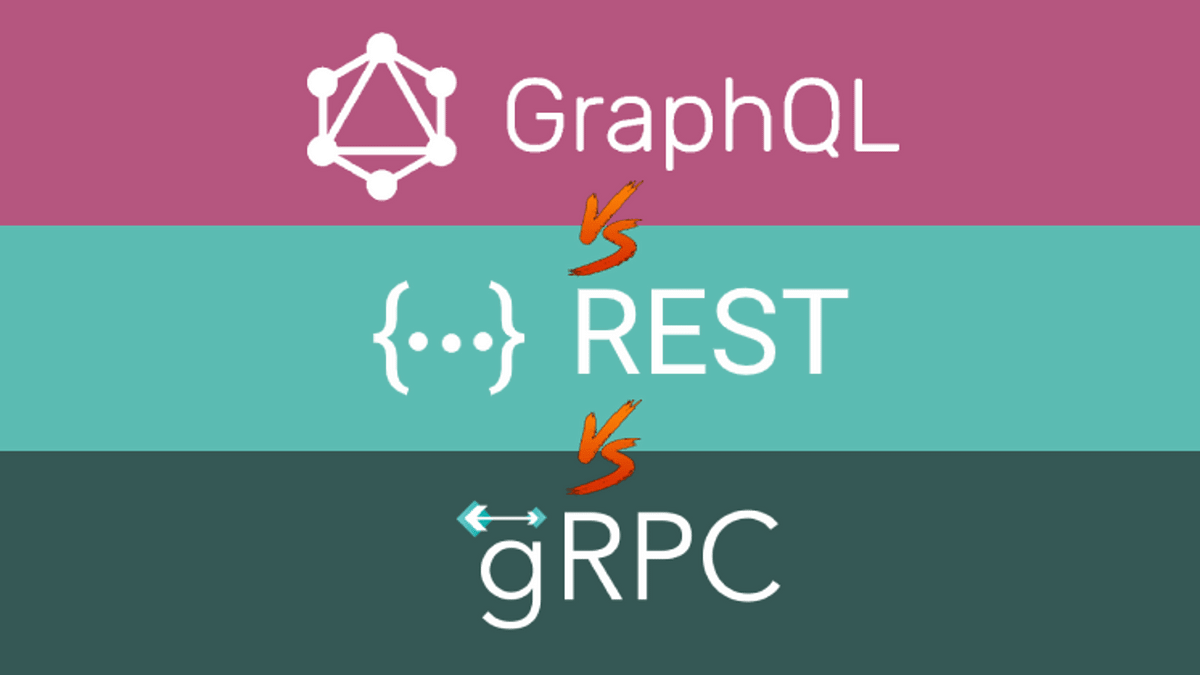
\includegraphics[width=\textwidth, height=0.6\textheight]{img/api-protocols.png}
    \end{center}
  \end{minipage}
  
  \vspace{15mm}
      \tiny { source: \href{https://mobilelive.medium.com/rest-vs-graphql-vs-grpc-comparing-three-modern-api-technologies-9ba58abadd82}{\textcolor{blue}{REST vs GraphQL vs gRPC: Comparing Three Modern API Technologies}}}

\end{frame}

\begin{frame}[fragile,t]{Understanding APIs \small (HTTP1 vs HTTP2)}  
	\begin{table}[t]
	\tiny
	\centering
		\begin{tabular}{  | >{\centering\arraybackslash}m{5cm} | >{\centering\arraybackslash}m{5cm} | }
		\hline
		\textbf{HTTP/1.1} & \textbf{HTTP/2} \\
		\hline
		Text-Based Protocol: Data is sent in a text-based format. & Binary Protocol: More efficient binary protocol, easier to parse. \\
		\hline
		One Request Per Connection: Each TCP connection allows only one request-response cycle at a time. & Multiplexing: Multiple requests and responses can be handled over a single TCP connection in parallel. \\
		\hline
		Headers Uncompressed: Headers are sent in plain text and can be quite large. & Header Compression: Uses HPACK compression to reduce overhead. \\
		\hline
		No Push Capabilities & Server Push \\
		\hline
		\end{tabular}
		\end{table}
    \begin{center}
      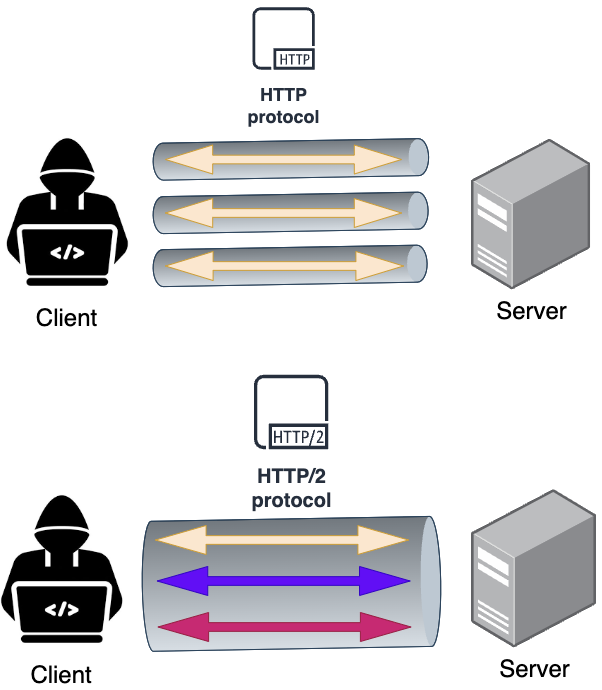
\includegraphics[width=0.6\textwidth, height=0.57\textheight]{img/http1-http2.png}
    \end{center}
  
\end{frame}

\begin{frame}[fragile,t]{Understanding APIs \small (gRPC Protocol)}  
	
	\begin{itemize}
	\scriptsize
      \item gRPC is a modern open source high performance Remote Procedure Call (RPC) framework that was developed in Google.
      \item gRPC can use \textbf{protocol buffers} as its underlying message interchange format.
      \item gRPC is based around the idea of defining a service, specifying the methods that can be called remotely with their parameters and return types.
      \tiny
      \item On the server side, the server implements this interface and runs a gRPC server to handle client calls. 
      \item On the client side, the client has a stub (referred to as just a client in some languages) that provides the same methods as the server.
    \end{itemize}
    
    \begin{center}
      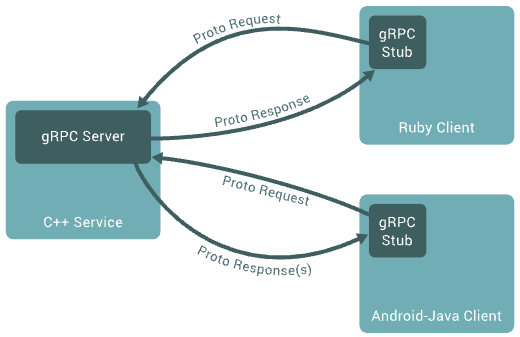
\includegraphics[width=0.5\textwidth, height=0.4\textheight]{img/grpc.png}
    \end{center}
    
    \tiny { source: \href{https://grpc.io/docs/what-is-grpc/introduction/}{\textcolor{blue}{Introduction to gRPC}}}
  
\end{frame}

\begin{frame}[fragile,t]{Understanding APIs \small (Protocol Buffers)}  
	
	\begin{itemize}
	\scriptsize
      \item Protocol Buffers are a language-neutral, platform-neutral extensible mechanism for serializing structured data.
      \item The file that includes the definition is \code {.proto} file
      
      \item[] 
      \scriptsize
      \begin{lstlisting}[language=protobuf]
		message Person {
			string name = 1;
			int32 id = 2;
			bool has_kids = 3;
			optional string email = 4;
		}
      \end{lstlisting}
    \end{itemize}
    
    \begin{center}
      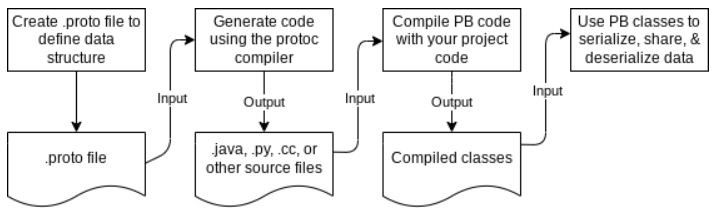
\includegraphics[width=0.7\textwidth, height=0.3\textheight]{img/protobuf-img.png}
    \end{center}
    
    \tiny { source: \href{https://protobuf.dev/overview/}{\textcolor{blue}{protobuf overview}}}
  
\end{frame}

 
 
\section{API Design Principles}
\begin{frame}{API Design Principles}
  \begin{itemize}
    \item Fundamentals of Good API Design
    \item Designing for Scalability and Performance
    \item API Versioning Strategies
  \end{itemize}
\end{frame}

\section{RESTful API Design}
\begin{frame}{RESTful API Design}
  \begin{itemize}
    \item RESTful Architecture Principles
    \item Designing RESTful Services (Endpoints, HTTP Methods, Status Codes)
    \item Best Practices in RESTful API
  \end{itemize}
\end{frame}



\section{Advanced API Protocols}
\begin{frame}{Advanced API Protocols}
  \begin{itemize}
    \item Introduction to GraphQL and Its Advantages
    \item Implementing gRPC for Microservices
    \item Comparison of Different API Styles
  \end{itemize}
\end{frame}

\section{API Documentation and Specification}
\begin{frame}{API Documentation and Specification}
  \begin{itemize}
    \item Importance of Comprehensive API Documentation
    \item Tools for API Documentation (Swagger, OpenAPI Specification)
    \item Maintaining and Versioning API Documentation
  \end{itemize}
\end{frame}

\section{API Security}
\begin{frame}{API Security}
  \begin{itemize}
    \item Authentication and Authorization Mechanisms (OAuth, JWT)
    \item Securing API Endpoints
    \item Handling Sensitive Data and Privacy Concerns
  \end{itemize}
\end{frame}

\section{API Testing and Quality Assurance}
\begin{frame}{API Testing and Quality Assurance}
  \begin{itemize}
    \item Writing Effective API Tests
    \item Tools and Frameworks for API Testing
    \item Performance Testing and Load Testing for APIs
  \end{itemize}
\end{frame}


\section{API Management and Lifecycle}
\begin{frame}{API Management and Lifecycle}
  \begin{itemize}
    \item The Lifecycle of API Development
    \item API Deployment Strategies
    \item Monitoring and Analytics for APIs
  \end{itemize}
\end{frame}

\section{Conclusion}
\begin{frame}{Conclusion}
  \begin{itemize}
    \item Recap of Key Learnings
    \item Emerging Trends in API Development
  \end{itemize}
\end{frame}

\end{document}
